% Preamble ==================================================================
\documentclass[11pt]{article}
\usepackage{geometry}
\geometry{verbose,tmargin=2.5cm,bottom= 1.5cm,lmargin=2.5cm,rmargin=2.5cm}
\usepackage{float}
\usepackage{graphicx}
\usepackage{amsmath}
\usepackage{amssymb}
\usepackage{enumitem}
\usepackage{mathtools}

\usepackage{amsthm} % theorem
\usepackage{listings} % code snippets
\usepackage{fancyvrb} %verbatim
\usepackage{xcolor}  % color math
\lstset{frame=l,
  language=Python,
  basicstyle={\small\ttfamily},
  numbers=none,
  numberstyle=\tiny\color{black},
  keywordstyle=\color{black},
  commentstyle=\color{blue},
  stringstyle=\color{mauve},
}

\numberwithin{equation}{section}

\usepackage{titlesec,dsfont}

%Format section heading style
\usepackage{sectsty}
\sectionfont{\sffamily\bfseries\large}
\subsectionfont{\sffamily\normalsize\slshape}
\subsubsectionfont{\sffamily\small\itshape}
\paragraphfont{\sffamily\small\textbf}


%Put period after section number
\makeatletter
\def\@seccntformat#1{\csname the#1\endcsname.\quad}
\makeatother

%Bibliography
\usepackage[round]{natbib}
\bibliographystyle{genetics}

%Format captions
\usepackage[ labelsep=period, justification=raggedright, margin=10pt,font={small},labelfont={small,normal,bf,sf}]{caption}

\setlength{\parskip}{0ex} %No space between paragraphs.

\renewcommand{\familydefault}{\sfdefault}

\newcommand\indep{\protect\mathpalette{\protect\independenT}{\perp}}
\newcommand{\nindep}{\not\!\perp\!\!\!\perp}
\def\independenT#1#2{\mathrel{\rlap{$#1#2$}\mkern2mu{#1#2}}}

%PUT ME LAST--------------------------------------------------
\usepackage[colorlinks=true
,urlcolor=blue
,anchorcolor=blue
,citecolor=blue
,filecolor=blue
,linkcolor=black
,menucolor=blue
,linktocpage=true
,pdfproducer=medialab
,pdfa=true
]{hyperref}

\makeatother %Put this last of all


\newcommand{\defeq}{\coloneqq}
\newcommand{\overbar}[1]{\mkern 1.5mu\overline{\mkern-1.5mu#1\mkern-1.5mu}\mkern 1.5mu}

% Make theorems bold
\makeatletter
\def\th@plain{%
  \thm@notefont{}% same as heading font
  \itshape % body font
}
\def\th@definition{%
  \thm@notefont{}% same as heading font
  \normalfont % body font
}
\makeatother

\newtheorem{thm}{Theorem}[section]
\newtheorem{defn}{Definition}[section]
\newtheorem{cor}{Corollary}[section]
\newtheorem{prop}{Property}[section]
\newtheorem{rle}{Rule}[section]
\newtheorem{lma}{Lemma}[section]

\definecolor{dred}{HTML}{c90404}
\definecolor{dgreen}{HTML}{0b8717}
\definecolor{dmagenta}{HTML}{c904c6}

%Preamble end--------------------------------------------------


\begin{document}

\begin{flushleft}
\textbf{\Large Geometric Deep Learning}
\end{flushleft}

\begin{flushleft}
Author: Juvid Aryaman

Last compiled: \today
\end{flushleft}

\noindent This document contains my personal notes on Geometric Deep Learning, largely based on \cite{Bronstein21}\footnote{See also \url{https://geometricdeeplearning.com/}}.

\section{High-dimensional learning}

We discuss the curse of dimensionality in supervised machine learning to motivate why inductive priors are helpful to construct. We'll consider the data domain to be $\mathbb{R}^d$ for this particular discussion.

\subsection{Notation}

\newcommand{\eloss}{\tilde{\mathcal{R}}}
\newcommand{\ploss}{\mathcal{R}}
\newcommand{\hypclass}{\mathcal{F}}

\begin{itemize}[noitemsep]
\item Data $\mathcal{D} = \{(x_i, y_i)\}_i$, drawn i.i.d.\ from an underlying data distribution $P$ over $\mathcal{X} \times \mathcal{Y}$.
\item Assume data generated by unknown function $y_i = f(x_i)$.
\item Assume $\mathcal{X} = \mathbb{R}^d$ and $\mathcal{Y} = \mathbb{R}$.
\item The model, or hypothesis class, is a subset $\hypclass \subset \{f: \mathcal{X} \rightarrow \mathbb{R} \}$.
\item The hypothesis class is assumed to come equipped with a complexity measure of all elements: $\gamma: \hypclass \rightarrow \mathbb{R}$. This can usually be defined as a norm, making $\mathcal{F}$ a \textbf{Banach space}.
\item The (convex) error metric $l(y, y')$, e.g. squared error $l(y,y')=|y-y'|^2$.
\item Loss. Consider $\tilde{f} \in \mathcal{F}$
	\begin{itemize}[noitemsep]
	\item Population loss: $\ploss(\tilde{f}) = \mathbb{E}_P[l(\tilde{f}(x), f(x))]$. This is the true loss of the hypothesis, averaged over the entire data domain.
	\item Empirical loss: $\eloss(\tilde{f}) = 1/n \sum_i l(\tilde{f}(x_i), f(x_i))$. This is the loss over some finite sample $\mathcal{D}$.
	\end{itemize}
\end{itemize}


\newcommand{\hypdelta}{\hat{f}}
\newcommand{\infimum}[1]{\underset{#1}{\text{inf}}}
\subsection{Empirical risk minimization}

The underlying goal in supervised learning is to minimise the population loss $\mathcal{R}(\tilde{f})$ given only access to the empirical loss. We seek to construct a bound for the population loss of a hypothesis. Consider $\hat{f} \in \hypclass_\delta$, where $\hypclass_\delta = \{f \in \hypclass; \gamma(f) < \delta\}$, i.e. a hypothesis with bounded complexity. We then decompose $R(\hypdelta)$ as follows:
\begin{align}
\color{dred}{\ploss(\hypdelta) - \infimum{f \in \hypclass} \ploss(f)} &= \textcolor{blue}{\left(\eloss(\hypdelta) - \infimum{f \in \hypclass_\delta} \right)} \textcolor{dgreen}{+ \left[\left(\ploss(\hypdelta) - \eloss(\hypdelta)\right) - \left( \infimum{f \in \hypclass_\delta} \ploss(f) - \infimum{f \in \hypclass_\delta} \eloss(f) \right) \right]} \nonumber \\
&\color{dmagenta}{+ \left( \infimum{f \in \hypclass_\delta} \ploss(f) - \infimum{f \in \hypclass} \ploss(f) \right)}
\end{align}
where
\begin{itemize}
\item The {\color{dred}{red}} term is the population loss of the hypothesis $\hypdelta$ relative to the best-possible hypothesis in the hypothesis class $\hypclass$.
\item The {\color{blue}{blue}} term is the {\color{blue}{optimization loss}}, i.e. how close the empirical loss of the hypothesis gets to the best possible hypothesis in the ball of hypotheses considered $\hypclass_\delta$. Call this $\epsilon_\text{opt}$.
\item The {\color{dgreen}{green}} term is the {\color{dgreen}{statistical error}}, denoting noise from the finite sample used to evaluate the empirical loss, relative to the sampling noise from the best hypothesis in the ball. This can be bounded from above by [\textbf{TODO: Didn't understand how}]
\begin{equation}
\epsilon_\text{stat} = 2\underset{f \in \hypclass_\delta}{\text{sup}} |\ploss(f) - \eloss(f)|
\end{equation}
\item The {\color{dmagenta}{magenta}} term is the {\color{dmagenta}{approximation error}}, denoting how close the constrained hypothesis class can get to the best function in the unconstrained hypothesis class. Call this $\epsilon_\text{approx}$.
\end{itemize}
Thus
\begin{equation}
\ploss(\hypdelta) \leq \infimum{f \in \hypclass} \ploss(f) + \epsilon_\text{opt} + \epsilon_\text{stat} + \epsilon_\text{approx}.
\end{equation}
If the hypothesis class is dense then the infimum term is 0, e.g. neural networks with non-polynomial activation (Universal Approximation Theorems). Generally, as the approximation error reduces (through a larger hypothesis space, increasing $\delta$), the statistical error increases. 

\subsection{Learning Lipschitz functions}
\begin{defn}[Lipschitz function]
A function $f: \mathcal{X} \subseteq \mathbb{R}^d \rightarrow \mathbb{R}$ is $\beta$-Lipschitz if 
\begin{equation}
|f(x)-f(x')| \leq \beta ||x-x'||
\end{equation}
i.e. the function cannot vary ``too quickly''. 
\end{defn}
If $f$ is 1-Lipschitz, and $P=\mathcal{N}(0, I_d)$, and using empirical risk minimization of the previous section, then a lower-bound on the amount of data required to estimate $f$ up to error $\epsilon$ grows as $\epsilon^{-d}$. The curse of dimensionality also crops up in e.g. using a single-layer perceptron to approximate a high-dimensional function, where the statistical error is cursed by dimension. 

However, in most cases, data are not simply points in a high-dimensional space: rather, the are \textbf{signals} on a low-dimensional \textbf{manifold} embedded in a high-dimensional input space $\mathcal{X}$ (Fig.~\ref{fig:geom-func-spaces}). The aim of an inductive prior (which is what Geometric Deep Learning is all about) is to reduce the statistical error, whilst keeping the approximation error low, by limiting ourselves to hypothesis spaces which respect the symmetries of the data domain.

\begin{figure}
\begin{center}
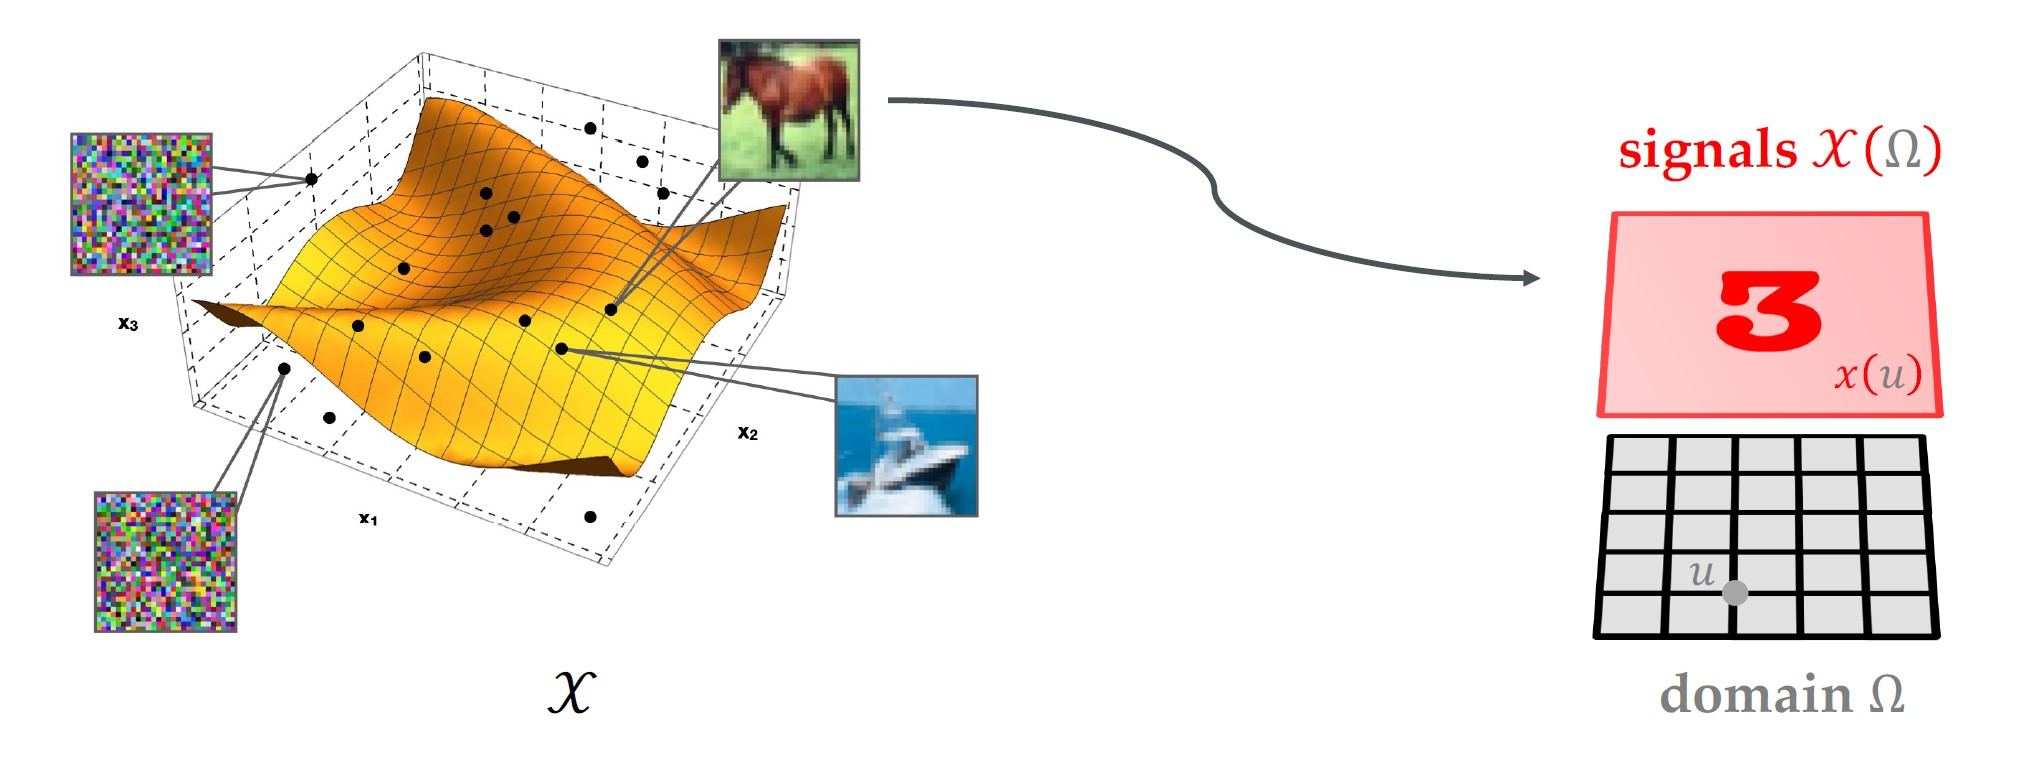
\includegraphics[width=0.8\columnwidth]{../figures/geometric-function-spaces.jpg}  
\end{center}
\caption{Geometric function spaces will allow us to exploit an underlying low-dimensional structure in the high-dimensional input space $\mathcal{X}$. For example, the space of all possible images are high-dimensional, but ``interesting'' images will exist on a lower-dimensional manifold embedded in the space of all images. Images off-manifold will look like boring noise. Geometric Deep Learning argues that data will often exist either on a grid, a graph, a group, or a manifold. Each of these have corresponding symmetries which can be leveraged.
}
\label{fig:geom-func-spaces}
\end{figure}

\newpage
\bibliography{geometric-dl.bib} 

\end{document}